
    \chapter{Introduction}
	
	\section{Motivation}
		
	Any task to make a prediction by combining data from different sources uses data fusion. Data fusion combines the information from multiple sources to achieve improved performance and inferences. According to Hall and Llinas [1] data fusion can be defined as “data fusion techniques combine data from multiple sensors and related information from associated databases to achieve improved accuracy and more specific inferences than could be achieved by the use of a single sensor alone.” The living organisms fuse information from various sources and past data to make an informed decision \cite{01_mandic2005data}. The data sources can be from various fields or different data types. Data fusion is described in different contexts and in other application areas. The most common areas include decision fusion and multisensor data fusion. [2]
	
	\begin{figure}[h]
		\centering
		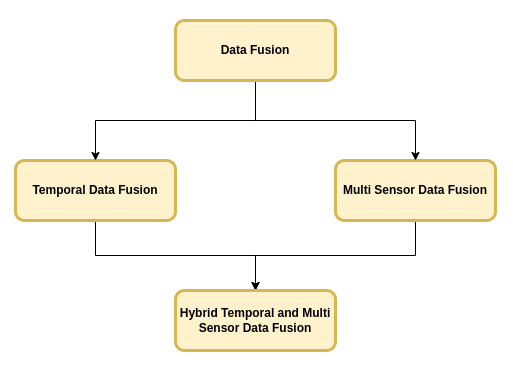
\includegraphics[width=10cm]{images/df.png}
		\caption{Data fusion categories based on timestamp}
		\label{fig:3D_reconstruction}
	\end{figure}

	Data fusion is divided into temporal and current data based on the timestamp factor. Temporal data are the data collected from the former steps. In the current data fusion approach, the data are extracted from the current step and are fused for improved prediction.Information fusion is applied in different fields such as time series prediction \cite{02_lim2021temporal}, video-based depth estimation \cite{03_duzceker2021deepvideomvs}, and segmentation \cite{04_li2021spatial}.
	
    Understanding surrounding regions and decision making of a human is based on the signals obtained from different sensors. However, with the knowledge of the past helps to better recognize the nearby activity or to make a educated choice. Thereby fusing the information from different sources and the former data adds to achieve a improved outcome. Temporal fusion is a process of fusing the information to the current step to make the prediction better at each timestamp. Common temporal data types include weather data, frames in a video sequence, and different sensor data. Semantic segmentation take advantage of the temporal fusion to make a better decision. 
    
    \subsection{Temporal fusion}

    In a general setting the previous data is not utilized to make a current prediction, resulting in information loss. The rich features from the past can be utilized in the current step, thereby making a robust and efficient model prediction. 

    \subsection{Semantic segmentation}
	
	Semantic segmentation is a process of classifying the each pixel of the input frame into a predefined specific class.  

    \section{Challenges and Difficulties}
    \subsection{...}

    \lipsum[11-15]

    \subsection{...}

    \subsection{...}



    \section{Problem Statement}
    \subsection{...}

    \lipsum[21-30]

    \subsection{...}


    \subsection{...}
